\documentclass[blues]{poster}
\usepackage[A1,portrait]{vmargin}
\usepackage[english]{babel}
\usepackage[mathletters]{ucs}
\usepackage[utf8x]{inputenc}
\usepackage{wrapfig}
%\usepackage{tikz}

\let\eps=\varepsilon
%\let\phi=\varphi
%\let\rho=\varrho
%\def\theta{{\vartheta₀}}
%\def\xstrut{\vrule width0pt height2.5ex depth1.0ex\relax}

\makeatletter
\@definecounter{romlist}
\def\romlist{\edef\@romlistctr{romlist}
    \par\unskip
    \begingroup
    \parskip=0pt
    \list{\csname label\@romlistctr\endcsname}
         {\usecounter{\@romlistctr}%
          \def\makelabel##1{\hss\llap{##1}}}%
          \setlength\itemsep{0pt}%
          \setlength\parsep{0pt}%
       }
\def\endromlist{\endlist\endgroup}
\def\labelromlist{\textbullet}
\def\theromlist{\arabic{romlist}}
\def\@authorboxwidth{50cm}
\makeatother

\setmargnohfrb{1.8cm}{1.8cm}{1.8cm}{1.8cm}%
\newcommand{\SiTiO}{Si$_x$Ti$_{1-x}$O$_2$}

\begin{document}
\title{Composition induced changes in optical response of Si-doped titanium dioxide}
\affiliation
  {\hsize=18cm
   \hbox{
\includegraphics[height=4.2cm]{MU-blue.pdf} \quad
	
\includegraphics[height=3.8cm]{OPVK_hor_zakladni_logolink_RGB_eng.jpg}}
   \hbox{
\includegraphics[height=4.2cm]{MUL.jpeg}\quad
		 
\includegraphics[height=4.0cm]{University_of_Nantes.pdf}
         
\includegraphics[height=4.2cm]{CEITEC.pdf}}
	}
  {\authorbox
   {Pavel Ondračka $^{a,b}$, David Holec $^c$, Daniel Franta $^{a}$,\\
	Eva Kedroňová $^{a,b}$, Stéphane Elisabeth $^d$,\\
	Antoine Goullet $^d$, Lenka Zajíčková $^{a,b}$}
   {$^a$ Faculty of Science, Masaryk University, Kotlářská 2, 611 37 Brno, Czech Republic\\
	$^b$ CEITEC - Central European Institute of Technology, Masaryk University, Kotlářská 2, 611 37 Brno, Czech Republic\\
	$^c$ Department of Physical Metallurgy and Materials Testing, Montanuniversität Leoben,\\
		Franz-Josef-Straße 18, Leoben A-8700, Austria\\
	$^d$ Institut des Matériaux Jean Rouxel (IMN), Université de Nantes,\\
		UMR CNRS 6502, 2 rue de la Houssinière, BP 32229, 44322 Nantes Cedex 3, France
	}
}

\vskip-1ex
\hrule height0pt

\begin{multicols}{2}

\subsection{Introduction and methodology }

\begin{wrapfigure}{r}{0.30\linewidth}
  \vspace{-20pt}
  \begin{center}
    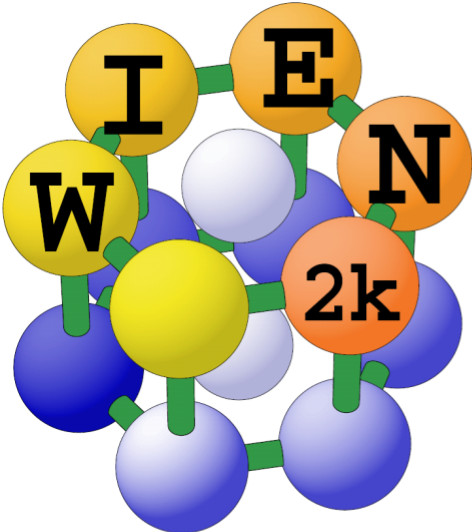
\includegraphics[height=3cm]{WIEN2k-logo.jpg}
    
\includegraphics[height=3cm]{VASP-logo.jpg}
  \end{center}
  \vspace{-20pt}
\end{wrapfigure}

\emph{Titanium dioxide} (TiO$_2$) thin films are extensively studied because of their interesting optical, electrical and
chemical properties. TiO$_2$ has a notably high refractive index and a high static dielectric constant. 
Alloying Si into TiO$_2$ can be used to fine tune its optical properties and to help to overcome some of TiO$_2$ films shortcomings, such as the columnar morphology, which leads to increased optical losses and degradation of its insulating character.

In the present work, the variation of Si$_x$Ti$_{(1-x)}$O$_2$ optical constants with the Si concentration are examined by employing \emph{Density Functional Theory}. 
The \emph{Special Quasi-random Structure} method is used to generate structural models of Si$_x$Ti$_{(1-x)}$O$_2$ disordered states for $x$=0.0625, 0.125, 0.1875, 0.25, 0.5, 0.75 and 1 for \emph{anatase} and \emph{rutile} phases. These initial supercells are structurally optimized using the Vienna \textit{Ab initio} Simulation Package. 
Optical constants of the resulting structures are calculated by the linearized augmented plane wave method as implemented in the Wien2k full potential all electron code together with the recently developed \emph{modified Becke-Johnson exchange-correlation potential} (mBJ).

Calculations are compared with experimental data obtained by \emph{ellipsometry and spectrophotometry} performed on Si$_x$Ti$_{(1-x)}$O$_2$ samples deposited by plasma-enhanced chemical vapor deposition (PECVD). Stochiometry of PECVD films was determined by XPS.


\subsection{Band gap evolution}

\begin{minipage}{0.4\linewidth}

\begin{itemize}
\item{Much better agreement between experimental and calculated band gap with mBJ compared to conventional LDA or GGA}
\item{Bang gap decreases slightly between $x = 0$ and $x = 0.5$, then it increases sharply}
\item{Calculated band gap evolution trend matches our experimental data}
\item{Calculated band gap of amorphous cells underestimated}
\end{itemize}

\end{minipage}
\begin{minipage}{0.6\linewidth}   

\includegraphics[width=\linewidth]{figures/gap.pdf}
\end{minipage}


\vspace{-0.5cm}
\subsection{Band structure evolution}
\includegraphics[width=\hsize]{figures/SiTiO2-dos.pdf}

\subsection{Evolution of optical constants}

\includegraphics[width=\hsize]{figures/n-anatase.pdf}

\includegraphics[width=\hsize]{figures/SiTiO2-eps.pdf}


\includegraphics[width=\hsize]{figures/compare.pdf}

\begin{itemize}
\item{Very good match between experimental and calculated anatase $\eps_\mathrm{i}$ for $x = 0$ and $E < 6$\,eV}
\item{Calculated $\eps_\mathrm{i}$ is too high for energies above 6\,eV and $x > 0$ which results in mismatch of experimental and calculated refractive index}
\end{itemize}

\subsection{Dielectric function near absorption onset}

\begin{minipage}{0.5\linewidth}   

\begin{itemize}
\item{Downshift of the absorption edge with increasing Si content}
\item{Very weak absorption near the absorption edge could explain the difference between calculated and experimental band gap}
\item{Silicon-induced oxygen defect states appear at the top and bottom of the valence band}
\item{Amorphous mixtures does not show this behaviour}
\end{itemize}

\end{minipage}
\begin{minipage}{0.5\linewidth}
\includegraphics[width=\linewidth]{figures/near-gap-eps.pdf}
\end{minipage}

\renewcommand{\familydefault}{\sfdefault}
\normalfont

\begin{center}
Bandstructure plots for Si$_{0.0625}$Ti$_{0.9375}$O$_2$
\end{center}

\vspace{-0.3cm}
\begin{minipage}{0.5\linewidth}
\begin{center}
\hspace{1.3cm}Bandcharacter for O near Si site\vspace{0.1cm}
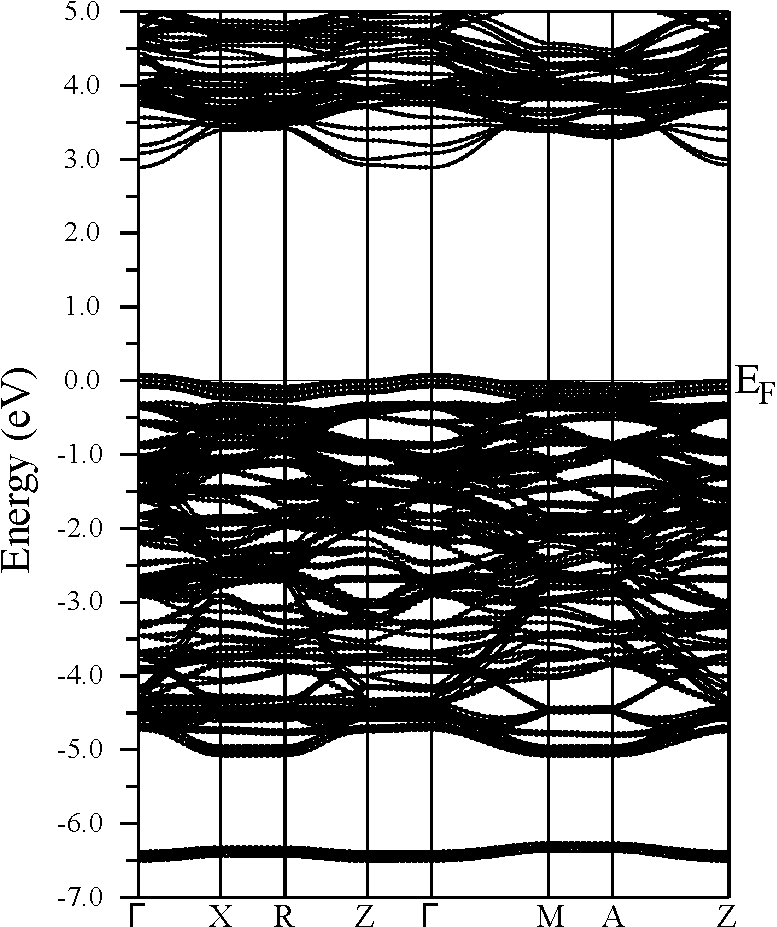
\includegraphics[height=16cm]{figures/spaghettiOSi.pdf}
\end{center}
\end{minipage}
\begin{minipage}{0.5\linewidth}
\begin{center}
\hspace{0.3cm}Bandcharacter for O away from Si site\vspace{0.1cm}
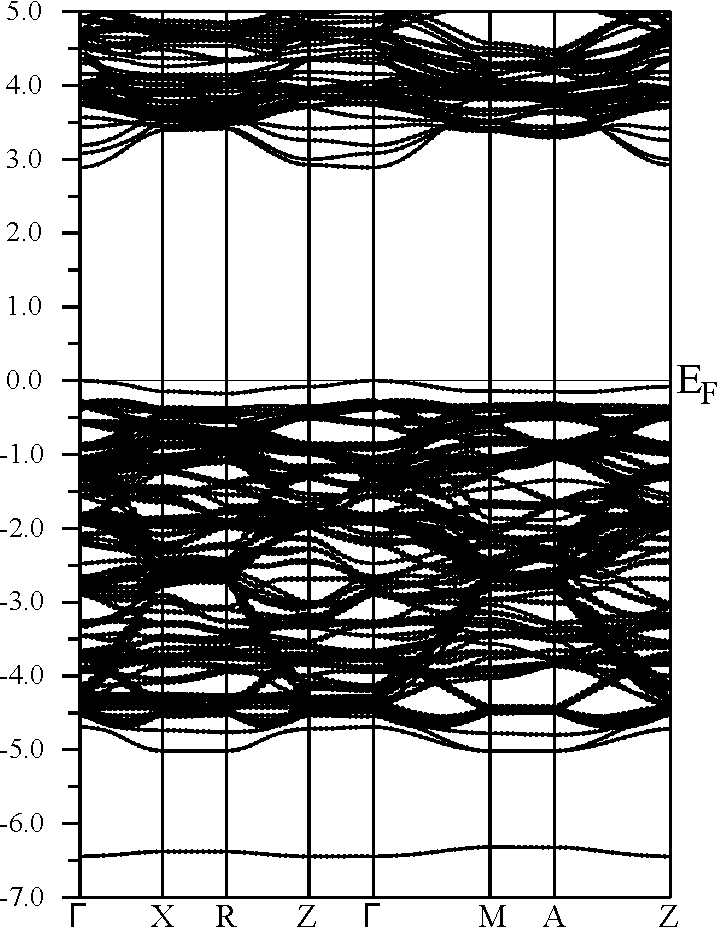
\includegraphics[height=16cm]{figures/spaghettinotOSi.pdf}
\end{center}
\end{minipage}

\renewcommand{\familydefault}{\rmdefault}
\normalfont

\vspace{-0.5cm}
\subsection{Conclusions}
\begin{itemize}
\item{mBJ potential results in a good agreement between the calculated and experimental band gap.}
\item{A good match between the calculated and experimental $\eps_\mathrm{i}$ especially for $x = 0$ and $E < 6$\,eV.}
\item{Interesting behavior near the absorption edge due to the silicon induced oxygen states.}
\end{itemize}

\vspace{-0.5cm}
\subsection{Acknowledgment} This work was supported by the IT4Innovations Centre of Excellence project (CZ.1.05/1.1.00/02.0070), funded by the European Regional Development Fund and the national budget of the Czech Republic via the Research and Development for Innovations Operational Programme, as well as Czech Ministry of Education, Youth and Sports via the project Large Research, Development and Innovations Infrastructures (LM2011033), by the project
,,Science and Scientists for Education of Modern Society'' (Grant No.
CZ.1.07/2.3.00/35.0005) co-financed by the European Social Fund and the State
Budget of the Czech Republic and by the ,,Erasmus'' programme.

\end{multicols}
\end{document}
